\documentclass[12pt,draftcls,onecolumn]{IEEEtran}
%\documentclass[onecolumn]{IEEEtran}

\usepackage{amsmath}
\usepackage{amsthm}
\usepackage{amssymb}  % assumes amsmath package installed
\usepackage{algorithmic}
\usepackage{algorithm}
\usepackage{cite}
\usepackage{color}
\usepackage{comment}
\usepackage{epsfig}
\usepackage{float}
\usepackage{graphicx}
\usepackage{multicol}
\usepackage{subfigure}
\usepackage{setspace}
\usepackage{comment}
\usepackage{subfig} % for subfigures
\usepackage{caption}

\newtheorem{theorem}{Theorem}[section]
\newtheorem{lemma}[theorem]{Lemma}
\newtheorem{proposition}[theorem]{Proposition}
\newtheorem{corollary}[theorem]{Corollary}
\newtheorem{remark}[theorem]{remark}

\begin{document}

\title{Progress Report on the Path Planning of Webot Satisficing Experiment }


\author{  Min Zheng \\  \today}

\date{\today}

% make the title area
\maketitle



%\IEEEpeerreviewmaketitle

%%%%%%%%%%%%%%%%%%%%%%%%%%%%%%%%%%%%%%%%%%%%%%%%%%%%%%%%%%%%%%%%%%%%%%%%%%%%%%
This project considers the integrated navigation and control of an unmanned ground vehicle(UGV) deployed to visually classify multiple targets in an obstacle-populated environment. 
This report describes the setup of the path planning problem and proposes some potential problems and plans. 

\section{Workspace construction} 

The workspace is the same as the one used for active satisficing human studies. 
The UGV and 30 target objects are in the same environment that consists of four rooms, denoted as the region-of-interest (ROI).
Similar to the human studies, there are 30 targets, denoted as $\mathcal{T} = \{\mathcal{T}_i; i = 1,2,...30; \mathcal{T} \subset W \}$.
The targets are considered as points.

A two-dimensional representation from the webot environment was extracted, and the workspace is constructed in MatLab, as shown in the figure below  (Figure \ref{fig:2}). 
The construction of workspace is built in an object oriented manner with classes of obstacles, targets and robot, each has properties and functionalities.  




\begin{figure}[p]
\centering
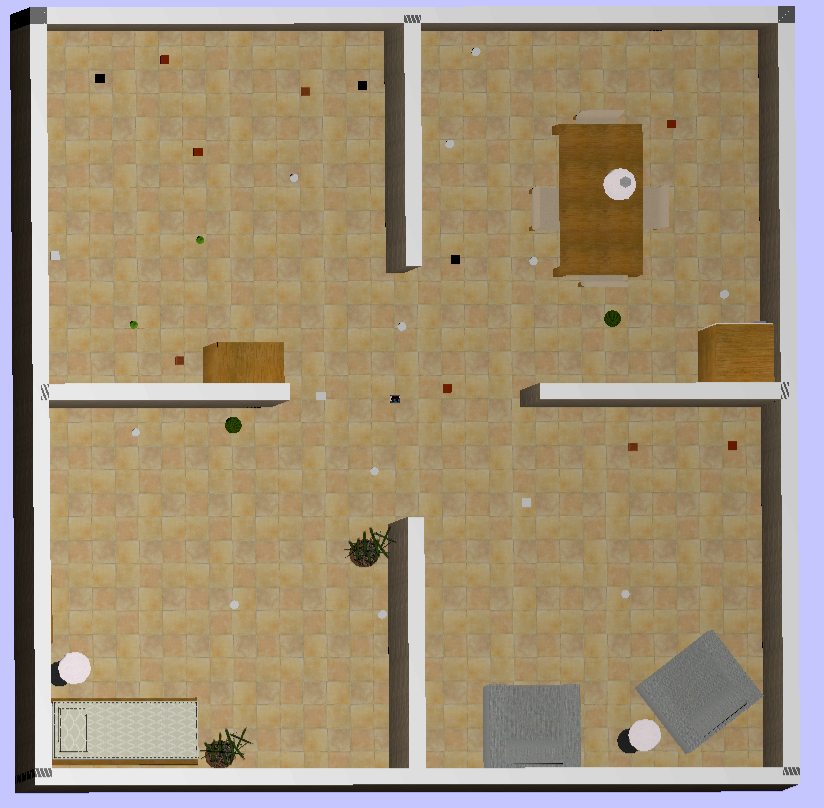
\includegraphics[width=10cm]{figures/webotTop}
  \caption{Top view of the webot environment}
  \label{fig:1}
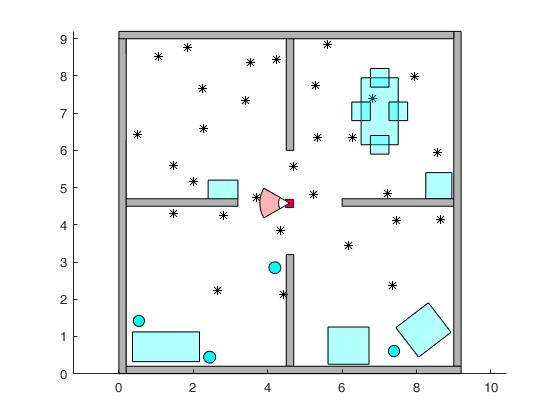
\includegraphics[width=16cm]{figures/matlabExtraction}
  \caption{2D representation built in MatLab. Obstacles are represented by colored regions, and targets represented by the stars. The UGV is  the red square, while its FOV is the red area within the fan shape.}
  \label{fig:2}
\end{figure}



\clearpage


\section{FOV and C-Target generation} 


The UGV sensor in the webot environment has platform geometry $\mathcal{A}$, and FOV geometry $S \subset \mathbb{R}^2 $. 
In order to combine with Zeyu's visual classification project, the FOV was determined based on requirement of  images taken. 
A successful classification requires the image to be taken within a minimum and a maximum distance, denoted by $d_{min}$ and  $d_{max}$. 
The on board camera has the same open angle $\theta$ as the human tests. 
Currently, the UGV is simplified to have no rotation, but only translation.
Therefore, the camera will always point to the same direction. 
 

C-Target is defined so that the target $\mathcal{T}_i$ in $\mathcal{W}$ maps  in the robot's configuration space  $\mathcal{C}_{free}$ to the C-target region  $\mathcal{CT}_i = \{q \in \mathcal{C}_{free}    |    \mathcal{S}(q) \cap \mathcal{T}_i  \neq  \emptyset \}$.
Based on the FOV described above, C-Target is plotted in the workspace (Figure \ref{fig:4}).
C-Target is denoted by white, where the rest region in $\mathcal{C}_{free}$ is grey. 
Currently, all of the obstacles are treated as not traversable. 
However, in the human tests, the UGV can go under the table and the chairs. 
Also, with the previous assumption that the UGV does not rotate, some of the targets are made impossible to measure given a particular camera direction, such as the red star in Figure \ref{fig:4}. 



\begin{figure}
 \centering
  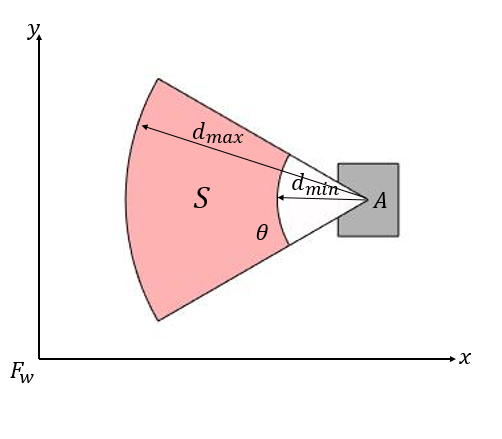
\includegraphics[width=10cm]{figures/FOV}
  \caption{FOV of the UGV}
  \label{fig:boat1}
\end{figure}


\begin{figure}
 \centering
  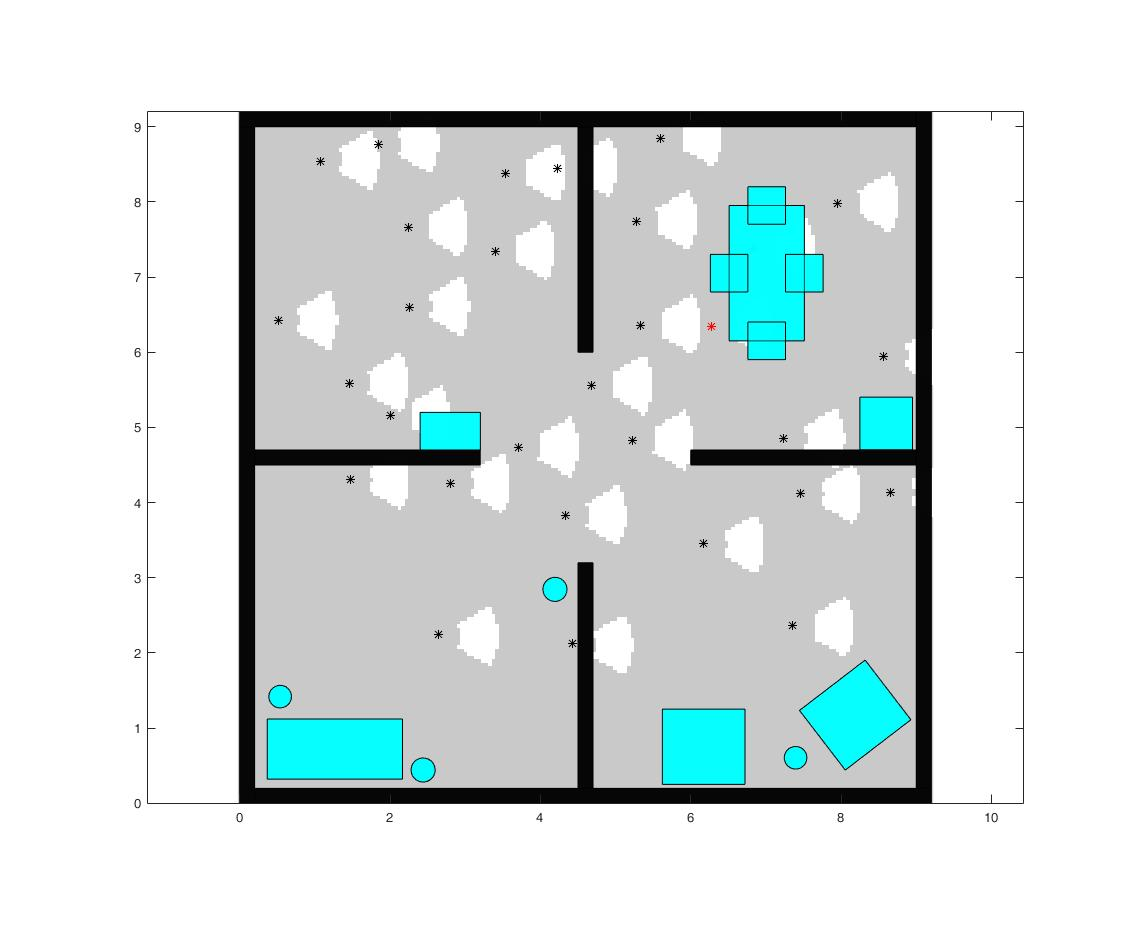
\includegraphics[width=18cm]{figures/CTarget}
  \caption{C-Target is denoted by white, where the rest region in $\mathcal{C}_{free}$ is grey.}
  \label{fig:4}
\end{figure}

\section{Next step} 
In the next step, the EER based on initial cues of the targets should be added, as well as a combination of uniform PDF and a Gaussian PDF.
After the hybrid PDF is obtained, the milestone can be generated to construct the roadmap.




\end{document}
